\documentclass{IEEEtran}
\usepackage{cite}
\usepackage{amsmath,amssymb,amsfonts}
\usepackage{algorithmic}
\usepackage{graphicx}
\usepackage{textcomp}
\def\BibTeX{{\rm B\kern-.05em{\sc i\kern-.025em b}\kern-.08em
    T\kern-.1667em\lower.7ex\hbox{E}\kern-.125emX}}
\begin{document}
\title{Preparation of Papers for IEEE TRANSACTIONS and JOURNALS (February 2017)}
\author{First A. Author, \IEEEmembership{Fellow, IEEE}, Second B. Author, and Third C. Author, Jr., \IEEEmembership{Member, IEEE}
\thanks{This paragraph of the first footnote will contain the date on 
which you submitted your paper for review. It will also contain support 
information, including sponsor and financial support acknowledgment. For 
example, ``This work was supported in part by the U.S. Department of 
Commerce under Grant BS123456.'' }
\thanks{The next few paragraphs should contain 
the authors' current affiliations, including current address and e-mail. For 
example, F. A. Author is with the National Institute of Standards and 
Technology, Boulder, CO 80305 USA (e-mail: author@boulder.nist.gov). }
\thanks{S. B. Author, Jr., was with Rice University, Houston, TX 77005 USA. He is 
now with the Department of Physics, Colorado State University, Fort Collins, 
CO 80523 USA (e-mail: author@lamar.colostate.edu).}
\thanks{T. C. Author is with 
the Electrical Engineering Department, University of Colorado, Boulder, CO 
80309 USA, on leave from the National Research Institute for Metals, 
Tsukuba, Japan (e-mail: author@nrim.go.jp).}}

\maketitle

\begin{abstract}
Software Defined Networking (SDN) is a promising paradigm that enables flexible management for networks by decoupling the control plane from the data plane. It allows to centrally control the network through one or multiple controllers. However, deciding about the number of controllers to deploy in a network and their locations is a particular task which can directly affect the overall network performance. This problem is widely investigated in the literature and the existing evaluations are  varied and diversified. To facilitate the understanding of the problem, this work aims to synthesize the existing solutions to outline the state-of-the-art and identify limitations and future scope. Based on a conceptual evaluation model, the Systematic Literature Review (SLR) method is employed to collect relevant works investigating the Controller Placement Problem (CPP). This review systematically evaluates research on CPP based on questions formulated for this purpose. It classifies the existing solutions based on different criteria, discusses the limitations of the proposed schemes, and points out the non-investigated scenarios related to the studied problem. This paper, which is, to the best of our knowledge, the first attempt of an SLR on CPP, can be a stable basis for potential researchers in this area to address the aforementioned problems.
\end{abstract}

\begin{IEEEkeywords}
Enter key words or phrases in alphabetical 
order, separated by commas. For a list of suggested keywords, send a blank 
e-mail to keywords@ieee.org or visit \underline
{http://www.ieee.org/organizations/pubs/ani\_prod/keywrd98.txt}
\end{IEEEkeywords}

\section{Introduction}
\label{sec:introduction}
\IEEEPARstart{T}he CPP was firstly introduced by Heller et al. in \cite{HeSh12}. The authors only focus on the propagation delay and present an exhaustive search to determine the optimal controller placement within the network topology. By analyzing the performance of controllers in different network topologies, the authors conclude that one controller is often enough to keep the latency at a reasonable rate. Many other works only target the latency as an optimization objective while placing the controller. However, though a single controller could be enough in most topologies \cite{HeSh12} from a latency point-of-view, many more controllers are necessary to meet resilience requirements. Moreover, the single point of failure is also a crucial factor in the one controller SDN network. This fact encourages researchers to investigate the multiple CPP, in the aim to optimize the network performance. Various works are existing with different optimization goals, such as latency, reliability, load balancing, cost, QoS, etc... 

\section{Systematic Literature Review}
A systematic review essentially provides an exhaustive summary of relevant literature for a specific field of study. It collects and critically analyses research studies according to a structured methodology to answer predefined research questions. As a result, a systematic review offers a firm foundation to a research topic and opens new approaches for further progresses in the concerning field of study. Based on the guidelines for performing SLR \cite{KiCh07}, we establish our review to identify, interpret and analyze all available evidence related to the controller placement problem in software defined networks.

\subsection{Research questions}
Corresponding to the main objective of this SLR that is to examine the proposed methods to solve the CPP and to show the different challenges and opportunities that are posed based on this problem, six research questions were formulated to guide the evaluation process step by step, as listed in Table \ref{tab:QRs}.

\begin{table}*[!h]
    \centering
    \begin{tabular}{l p{4.5cm} p{6cm} }
  \hline
  ID & Research Question & Main Motivation \\
  \hline
  RQ1 & What are the purposes of solving the CPP? & To identify the requirements, goals, and constraints of investigating the CPP. \\
  RQ2 & What are methods used to solve the CPP? & To identify the mathematical methods used to solve the optimization problem. \\
  RQ3 & How are the methods evaluated? & To describe the experimental process established to evaluate the methods. \\
  RQ4 & What are the experimental setup to evaluate the test scenarios? & To explore the different environments used to test the proposed methods. \\
  RQ5 & What are the case study assumptions? & To determine the nature of the proposed solution. \\
  RQ6 & What are the metrics evaluated by the proposed work? & To point out the metrics used to compare different evaluations. \\
  \hline
\end{tabular}
    \caption{Research questions}
    \label{tab:QRs}
\end{table}


\subsection{Research scope and strategy process}
This study focuses on the solutions proposed by the literature to optimally choose the minimum number of controllers required for an SDN network, to decide where to place the controller(s) in the network, and how many networking devices should be assigned to a given controller. Although the term "controller placement problem" started to gain popularity in 2012 with Heller et al. \cite{HeSh12}, Zhang et al. where the first authors to discuss the controller location in a network in 2011 \cite{ZhBe11}. So, the publication time span of our survey covers the papers from 2011 until the time of conducting the study. The most suitable search terms we used to conduct our study were: "controller placement", "SDN", "WAN", "facility location", "control management", "switch assignment", along with the metrics optimized in the studied problem such as: "reliability", "resilience", "QoS", etc. These keywords allowed us to form several search strings such as: ("controller placement" OR "control plane management" OR "switch assignment" OR  "resilience" OR "reliability" ) AND ("software-defined networking" OR "SDN" OR  "WAN"). 

The inclusion and exclusion criteria can be presented as:
\subsubsection{Exclusion criteria}
\begin{itemize}
    \item Publications that describe only theoretical discussions \cite{SoXi17}.
    \item Publications of same authors but in different journals or conferences and that propose the same solution with a little difference in the work presentation \cite{HuWa12,HuWe13,HuWa14}. Only one of different papers is studied.
    \item Reports and technical works that are not published in any conference or journal.
\end{itemize}


\subsection{Review results}
In this section, we present a meta-analysis and quantitative evaluation of the data provided by the search and after eliminating papers according to exclusion criteria. 


%\subsection{Approach}
%\begin{itemize}
%\item Presenting the SLR
%\item Keywords and research scope
%\item Article selection, inclusion and exclusion
%%\item Questions
%\end{itemize}
%\subsection{Questions to answer}
%\subsection{Main results}
%Quantitative presentation 
%%figure sur les années
%%Stats pour les papiers selon la critère optimisée et l'année

\section{Discussion Addressing Research Questions}
This section discusses the objectives and challenges faced by the collected research papers addressing the CPP. It is organized in the same order as the defined research questions and aims to propose different classifications of the analyzed works by answering the questions.

\subsection{RQ1: What are the purposes of solving the CPP?}
%Intro

In this section, we classify the most relevant papers in the literature, according to the criteria used to optimally place the controller in an SDN. Our classification is based on the objective function optimized in the CPP. Among each of these classifications, the papers are also categorized based on the optimization problem constraints.

\subsubsection{Latency}
Latency is one of widely used performance metrics in computer networks \cite{SiHa15}. It is defined as the delay that occurs in data communication over a network. In SDNs, frequent message exchanges between switches and controllers and between different controllers (if there are many) are essential to carry out most SDN functions, such as flow instantiation, state update, etc. Thus, network latency can be an important criterion to take into consideration when optimizing SDN networks, namely when optimizing the controller placement. The overall latency consists of packet transmission latency, propagation latency, switch queuing latency, and controller processing latency \cite{WaZh17}. The packet transmission latency is related to the packet size and the data-rate of the link. The propagation latency is proportional to the distance between two communication nodes. The switch queuing latency is the delay caused by a link congestion. The controller processing latency consists of the delay affected by the controller load. However, most of the works presented in the literature to solve the CPP investigate the case of Wide Area Networks (WANs), where only propagation and processing latencies dominate because of the relatively small control message size in SDN and the assumed large capacity of control links. In this section, we mainly present the papers proposing solutions to the CPP by minimizing the propagation latency between switches and controllers as well as inter-controllers latency. Other works that minimize the propagation latency along with processing latency are also presented.

In \cite{HeSh12}, the authors consider the switch-to-controller latency and propose an exhaustive research to find the optimal placement by directly considering the metrics on all possible combinations of controllers. Both average and worst-case latencies are minimized by investigating k-median and k-center problems, respectively. The proposed algorithm is evaluated on WAN networks selected from Topology Zoo and simulated in Matlab. The authors observe that the location and number of controllers depend on the simulated network's topology. They also note that the average latency with a random placement is 1.4 to 1.7 larger than that of the optimal placement, while this ratio is between 1.4 and 2.5 for worst-case latencies. 

The sum of switch-to-controller and inter-controllers distances is minimized in \cite{SaSa16}. The authors propose a spectral clustering algorithm that partitions the network into smaller domains based on the distance between nodes, to optimally place the controller. The proposed algorithm is compared to k-median and k-center algorithms. Simulations show that the graph partitioning technique performs better than the two other algorithms in terms of inter-controller latency as well as the number of nodes managed by each controller. 

A clustering algorithm is also proposed in \cite{WaZh17} to minimize the maximum latency between controllers and switches. The proposed approach, called Clustering-Based Network Partition Algorithm, iteratively partitions the network into different subnetworks. For each subnetwork, a centroid that has the minimum sum of physical distances to all nodes is selected. The performance of the proposed algorithm is evaluated in comparison to the k-center and k-means approaches. Simulations show that the proposed approach ensures smaller maximum latency between the controller and associated switches than the one achieved by both k-center and k-means.

In all of these papers, the propagation latency was optimized without taking into consideration any other performance metric as a constraint. However, Yao et. al  introduce in \cite{YaBi14} the capacitated controller placement problem (CCPP) minimizing the maximum latency between the switches and their assigned controller subject to the controller capacity. In their model, the controller load established by the processing of PACKET\_IN events, delivering the events to the applications, communicating with other controllers and maintaining the view of the local network partition, has to be maintained under a capacity limit. The problem being NP-hard, a capacitated k-center strategy based on the algorithm introduced in \cite{OzPi06} is proposed to solve it. An Integer Programming model is also used to find the minimal number of controllers with a specified radius, where the radius denotes the maximum propagation latency between switches and the assigned controller. According to simulations, the proposed strategy can reduce the number of controllers required to avoid overload as well as the load of the heaviest-load controller, when compared to the k-center algorithm. 
%Also, it has smaller radius than using dynamic controller provisioning or dynamic scheduling strategy in k-center placement.

The traffic load of switches in terms of number of flows is considered in \cite{HuJo15} while minimizing the propagation latency. The contribution of this paper includes two parts. In a first step, the proposed method partitions the network into sub-regions and the location of controllers is chosen such that the maximum number of switches can be operated and the maximum latency can be minimized,  using the Bowyer-Watson algorithm. In a second step, the proposed approach called LiDy, dynamically adapts the number of controllers as the traffic load of switches varies using a dynamic flow management algorithm. Simulations show that the proposed algorithm requires a lower number of controllers to balance the same traffic load compared to the scheme proposed in \cite{YaBi14}, ensuring better control plane utilization while maintaining the latency within a maximum bound. 

The drawback of LiDy being its complexity, Huque et al. present LiDy+ in \cite{HuSi17} to reduce the time complexity of their former solution, while achieving similar performance in terms of latency, controller utilization, power consumption, and cost. The main difference between the two algorithms leads in the manner to split the network into sub-regions. More specifically, LiDy+ runs the smallest enclosing risk algorithm which enables a lower complexity than the triangular decomposition proposed by LiDy. LiDy+ is also applicable at large-scale networks.

The controller capacity is also considered as a constraint in \cite{GaWa15} when minimizing the global propagation latency, i.e. the sum of switches to controllers latency and the inter-controllers latency. The authors propose a particle swarm optimization (PSO) algorithm to solve the problem. However, the evaluation of the proposed algorithm is not very clear since it is based on the comparison with other algorithms solving different objective functions. 

The weighted switch-to-controller latency is minimized in \cite{YaHo15}. The optimized metric includes the 'routing cost', i.e. the distance from switch to controller multiplied by the weight of the switch, which reflects the maximum throughput it can achieve. The work presented in this paper encompasses two steps. In a first step, the controller placement problem is investigated for a single domain, i.e. where only one controller exists. An evaluation on a single domain network containing 16 nodes is proposed, adopting the hop count as the routing cost. Simulations prove that the proposed method has smaller average flow set-up cost compared with the strategy in \cite{HeSh12}. 

However, the assignment of a controller between the switches in a static manner generates load imbalance in dynamic flow conditions. Consequently, the authors propose, in the second step, a dynamic switch migration algorithm for multiple SDN domains, in order to adapt to the flow dynamics and realize load balancing between controllers. To this aim, the network topology is firstly divided into several sub-domains with a single controller in each domain. The number of partitioned sub-domains is determined according to the capacity of the controller and the requests of each switch. Finally, a dynamic scheduling strategy is proposed to release the overload problem and realize the load balancing between controllers. More specifically, when a controller becomes overload, it can cooperate with its neighbor controller and migrate the boundary switches to the neighbor domain to reduce its own load. The performance of the proposed algorithm is evaluated in the NSFNET topology, composed of two domains. Simulation results prove that the switch migration algorithm insures better load balancing than static method. %However, no comparison to other algorithms in the dynamic case is presented. 


%KiRa16

\subsubsection{Resilience}
There are several definitions of resilience which differ more or less in their meanings. In the following, we shall adopt the definition proposed by \cite{StHu07}, which claims that   "resilience is the ability of the network to provide and maintain an acceptable level of service in the face of various faults and challenges to normal operation".  Any other sense considered in the contributions will be pointed out.

Although the CPP was assigned to Heller \cite{HeSh12}, the work in \cite{ZhBe11} which was published one year before Heller's paper, treats the same problem, i.e. controller location, but in the aim to maximize the network resilience. The authors propose a min-cut based graph partitioning algorithm for controller placement to maximize the resilience of the network. They consider different types of failures, namely links and nodes failures. The partitions are identified with minimum cuts across boundaries, i.e. insuring a minimum connectivity between clusters. After the partitioning, the controller is placed in the centroid of the partition to guarantee the shortest path length to all switches in the same cluster. The proposed approach is evaluated using a perl-based simulation tool. Simulations show the impact of controller placement on resilience, and prove that the proposed algorithm outperforms the random and greedy based placements in terms of failure probability in various topologies and that this improvement is more important with large-scale networks. 

The same problem is investigated in \cite{MuOl14}. Müller et al. propose "Survivor": a resilient framework which reinforces the connectivity between controllers and switches, taking more routes, avoiding the overload of the controller and improving the failover by composing a list of backup controllers for each device in the network. The proposed approach encompasses two phases: Firstly, the CPP is investigated, such that capacity constraints are satisfied and connectivity is maximized, by choosing positions that yield the highest number of node-disjoint paths between the controller and the switches. The problem is presented as an Integer Linear Programming (ILP), where the capacity is defined as the maximum number of requests that a controller can handle per second. Secondly, a list of backup controllers for each device in the network is specified. Two heuristics for selecting backups during failover are proposed: one based on proximity and the other based on residual capacity. This method is evaluated with various simulated topologies from Topology Zoo and compared to the algorithm proposed in \cite{ZhBe11}. Many improvements of "Survivor" are noted: (a) considering multiple paths, i.e. exploring path diversity during placement, which reduces the chance of connectivity loss; (b) taking into consideration the capacity to avoid controllers overload; (c) improving smart recovery mechanisms thanks to the proposed heuristic for selecting backups during failover.

Resilience is jointly optimized with switch-to-controller link length in \cite{ViMa16}. In this paper, two strategies for controller placement in the aim of providing protection against link and node failures while minimizing controller to switch latency  are proposed. In the first strategy, every node must be connected to its assigned controller over two disjoint paths. In the second one, every node must be connected to two different controllers over two disjoint paths. The main idea of this work is to consider planning of the backups paths in advance. An optimization problem to find a controller placement that jointly optimizes working and backup paths is investigated for the two strategies. The problem is formulated as a Mixed Integer Linear Programming and the optimal placement is found using the Gurobi solver. The evaluation of performance metrics in several topologies with tens of nodes shows that the working paths in the proposed strategies may be longer than in the unprotected case (without backup paths). This difference decreases as the number of controllers increases. Simulations also show that both strategies ensure lower control path loss and better control path availability than the unprotected case. The authors verify the feasibility of the solving time for the simulated topologies with single and double link failures. However, they note that this time is not suitable for online use. %However, this paper does not take into consideration the capacity constraints.

\subsubsection{Reliability} 
Reliability is a measure of service continuity referring to the probability that a system remains operable in a given time frame \cite{Rak15}. Due to nature of SDN, where control plane is separated from the data plane, this network architecture may present reliability problems when one of the components fails. To face this problem, several papers consider reliability to optimally solve the CPP. In particular, Hu et al. propose in \cite{HuWa12,HuWe13} an algorithm to determine how many controllers and how to connect them in order to optimize the reliability of the network. In this perspective, they introduce a metric called "the expected percentage of control path loss" and define it  as the number of broken control paths due to network failures. They define the control paths as the set of routes between controllers and switches as well as inter-controllers routes. The authors only analyze failure scenarios where at most one physical component fails at a time. They do not propose any control path protection mechanism assuming that when a physical component fails, the control paths traversing this component fail as well. The reliability-aware controller placement problem being NP-hard, two heuristics are proposed to solve the problem: l-w-greedy and simulated annealing. These algorithms are compared to an exhaustive approach, the brute force algorithm, as well as to a random placement algorithm. Simulations prove that the simulated annealing algorithm provides solutions that are close to optimal. In order to analyze the impact of controller number on reliability, the authors set fixed failure probabilities for each switch and each link. They observe that using too few or too many controllers reduces reliability. Simulations also show trade-offs between reliability and latencies in both topologies.

%LiLi16

\subsubsection{Cost}
Many other papers consider the deployment cost (CAPEX and OPEX) as a critical factor to decide about the controller placement. This was the optimized objective function in \cite{SaSt15}, subject to various constraints, such as the capacity and the flow-setup latency, which includes transmission, propagation and processing delays. The capacity includes the maximum number of packets sent by the switches the controller can process and the bandwidth that can be handled by the links between switches and controllers. The maximum number of connected switches and controllers to one controller is also maximized by the number of ports on that controller. The minimized cost includes the cost of installing a controller, the cost of linking controllers to the switches, and the cost for linking controllers together. The problem is formulated as a linear programming model and solved with the CPLEX optimizer. The authors observe a slight decrease in the deployment cost when the number of potential placement locations increases. However, only small size problems can be optimized within a reasonable amount of time with the proposed NP-hard problem resolution. 

The same criterion constitutes the objective of Rath et al. in \cite{RaRe14}. Firstly, the authors formulates a multi-objective optimization problem that minimizes a non-linear function of the number of controllers and cost (CAPEX and OPEX) associated with each controller, subject to controller utilization (processor or memory or flow) and delay (processing and propagation) constraints. However, obtaining a unique optimal number of controllers is not possible since the load in the network changes constantly. Consequently, the authors propose an individual optimization problem minimizing only the cost of a controller with the same constraints as the global problem. They argue to solve the global optimization once with an initial condition to determine the initial optimal number of controllers, and then to solve the individual problem at each controller when load changes. A non-zero-sum game is used to obtain the best solution of the individual problem. The proposed solution calls two other algorithms in the cases of under or over utilization of the controller playing the game. In the former case, the controller is deleted and one or more neighbor controllers can share its load. In the latter case, the current controller can either offload to a neighbor controller or initiate a new controller. The authors present some simulation results to demonstrate the usability of the proposed algorithms but they do not present any complexity analysis or comparison to other schemes.

With the same ambition of minimizing the deployment cost in a network, along with the minimization of the synchronization overhead between controllers, the authors in \cite{RoRu14} aim to limit the number of controllers per node as well as the overall number of controllers. The authors introduce the 'fault tolerant controller placement problem' minimizing the sum of costs of deploying controllers and serving switches, subject to a reliability constraint. A heuristic algorithm is proposed and questions about the number of controllers to deploy, their placements, the nodes to which they must be assigned to are explored for different topologies. Simulation results show that the answers are dependant on the network topology more than on the network size. They also indicate that each node is required to connect to just 2 or 3 controllers to provide more than five nines reliability.

This work was extended in \cite{RoRu16}. The authors change their way to decorate the graph while solving the optimization problem, and thus get to find all disjoint paths that contribute to network reliability. This result leads to fewer controllers in the topology and fewer connections between controllers and switches. The authors also evaluated their proposition by analyzing the controller load, other reliability levels, and the runtime of the heuristic algorithm. The new results point out that, regardless the topology, each node only needs to establish a connection with two controllers at maximum to achieve more than five nine reliability level, which outperforms the results in \cite{RoRu14} where some nodes require three connections. 

Bari et al. also consider the number of controllers and their placements in \cite{BaRo13} but in a dynamic way. They are the first authors to focus an entire paper on the dynamic provisioning of controllers in SDN. In this paper, they propose a framework for dynamically adapting the number of controllers and their locations according to network dynamics, while ensuring minimal processing delay and communication overhead at the controller due to synchronization and management workload. For this purpose, they investigate an optimization problem minimizing the total cost (statistics collection, flow setup, synchronization between controllers, and switch reassignment costs) subject to latency between a switch and its assigned controller and controller capacity constraints. The problem is formulated as an Integer Linear Program and two heuristics programmed in Python are proposed to find the optimal switch to controller assignment. The first one is a greedy approach based on knapsack problem, while the other is based on simulated annealing. The simulated annealing algorithm outperforms the greedy approach in both number of controllers and flow setup time, but it requires much more time to run. Both approaches succeed to find a right trade-off between flow setup time (processing time - the extreme case is when we have only one controller to all switches) and communication overhead (communication between controllers - the extreme case is when we have one controller to each switch). 

In \cite{ChWa15}, the authors introduce the QoS-guaranteed controller placement problem to minimize the number of controllers in a topology. The optimization problem is constraint by the response time of a controller, which consists of the round trip latency between the controller and a switch, and the service time of a controller which depends on the capacity and the workload of a controller. The authors compare three heuristic algorithms for various topologies form the Internet Topology Zoo: Incremental greedy algorithm, primal-dual-based algorithm, and network-partition-based algorithm. They demonstrate that the incremental greedy method slightly outperforms the other two methods. The incremental greedy algorithm selects first the controller which can serve the maximum number of switches. At each iteration, the switch with the minimal delay from the controller is assigned to it. This operation is repeated until the average response time of all switches reach the response time constraint. However, this algorithm does not have any theoretical performance guarantee to the generated results. In the second method, the problem is formulated into an integer program. The primal-dual method then finds the near optimal solution to the integer program by using linear relaxation and the duality of the original problem. However, the above algorithms do no have a global view of the whole network, and they create unbalanced placement between controllers. The authors then detail the network-partition-based algorithm, which divided the network into partitions in a way that the maximum delay between two switches is within the response time constraint. In each partition, the incremental greedy method is used to place the controller. Simulation results prove that the incremental greedy algorithm slightly outperforms the other two algorithms in terms of number of controllers, while the network partition algorithm costs less response time than the other two algorithms.

Despite the different formulation of the problem, the authors in \cite{LiWa15} also try to minimize the number of controllers by maximizing the utilization of each controller. They propose a network clustering particle swarm algorithm to optimally locate the controller, taking into consideration the propagation latency, the load of controllers and load balancing. The proposed algorithm combines the capacitated k-center, with the aid of a clustering algorithm, with Particle Swarm Optimization (PSO) which was used in \cite{GaWa15}. The presented scheme is compared to the k-center and the capacitated k-center algorithms. Simulation results show that the proposed algorithm can reduce the number of controllers when every controller avoid overload. Moreover, the proposed strategy presents a better control plane utilization than the other algorithms, along with better load balancing. The propagation delay obtained by the proposed algorithm is too close from the one obtained by the k-center algorithm. 


\subsubsection{Multi-objective optimization problems}
When several performance metrics are considered, there is usually no single best controller placement solution, but a trade-off between these metrics. For this, many papers present the CPP as an optimization problem with multi-objective function and try to find the best trade-off between the optimized metrics.

In \cite{HoHa13}, an exhaustive evaluation of multiple metrics is presented and the resilient Pareto-based Optimal Controller placement (POCO) is introduced. The proposed framework allows to investigate a multi-objective optimization problem, offering all possible solutions evaluated by all objectives, allowing to select afterwards the placement that is most adequate for each one needs. The optimization objectives addressed by the authors are maximum latency between nodes and controllers, inter-controller latency, load balancing between controllers and resilience. For resilience, the authors consider both tolerance on network disruption as well as controller failures. Simulations evince an improvement in calculation times, a more efficient use of memory and RAM.

The authors extend their work in \cite{HoHa14} where they present the POCO-PLC method applied to the CPP in a dynamic way in SDN networks. Their proposal enables real-time performance analysis, using the PlanetLab network programmed in Python that measures the latency between external nodes and latency between local nodes in real time, as well as the load on the CPU. Then "Planet Lab" dynamically chooses the controller closest to the node in terms of the latency. Since the controller assignment is dynamic, it allows comparing in real time the different locations of the controller with respect to the previous locations.

POCO, in its default configuration, performs an exhaustive evaluation of all possible placements. Thus, it is practically possible only for small and medium sized networks and cannot be feasible for large-scale or dynamic networks as it has high time and resource constraints such as processing and memory. 
Consequently, the authors in \cite{LaGe15} propose an heuristic extension of POCO, that is less accurate but yields faster computation time. The authors derive guidelines for deciding whether to use an exhaustive evaluation or to switch to an heuristic approach, according to different use cases and requirements. The heuristic algorithm proposed in this work is based on Pareto Simulated Annealing (PSA), a Multiobjective Combinatorial Optimization (MOCO) algorithm inspired by simulated annealing. The heuristic method analyzes the trade-off between the time and accuracy and takes the latencies of the nodes, the latencies between the controllers, failure tolerance in nodes , failure tolerance in links and the load balance. Simulation results show that this method is less precise but faster to determine the location of the controller.

In \cite{JaAh15}, another heuristic extension to POCO based on NSGA-II (Non-dominated Sorting Genetic Algorithm II)  mixed with Pareto Frontier is proposed. This genetic algorithm is normally used in discrete and continuous optimization problems and this model is applied to the controller location problem. Latency between switches and its assigned controllers, inter-controllers latency, as well as load balancing between controllers are considered. A Matlab simulation of the "Internet2 OS3E" topology is performed and the proposed algorithm is proved to be efficient for achieving a good approximation of the Pareto Optimal frontier considering these objectives. 

Many other works try to solve the multi-objective problem for large-scale networks, by proposing heuristic schemes. In \cite{VaMo18}, the authors propose a heuristic algorithm called Multi-Start Hybrid Non-dominated Sorting Genetic Algorithm (MHNSGA) to solve the multi-objective CPP. The proposed algorithm is an adaptation of an NSGA algorithm especially based on greedy initialization and multi-start mechanism. Controller to switch latency, inter-controllers latency, and load balancing between controllers are optimized. Both average and maximum values are considered for latencies. Compared to the framework POCO, the proposed algorithm is able to find near-optimal solutions with much less run time and memory and, unlike POCO, it can be applied to large-scale networks. However, for such large-scale instances, it is not possible to evaluate the accuracy obtained by any heuristic algorithm since we can not calculate the exact solution for the evaluated placements. For smaller network sizes, MHNSGA is compared to POCO over 40 graphs from the Internet Topology Zoo and it is shown to provide an efficient estimation and good convergence towards the real Pareto optimal set. Compared to other heuristics, namely PSA \cite{LaGe15} and PSO-CGLPP \cite{GaWa15}, MHNSGA converges faster and outperforms the two algorithms in most of the time.  

Although this unconstrained model considers many factors crucial to place SDN controllers, the authors also emphasize a different variant of the problem taking into consideration the controller capacity and the switch load. The constrained problem being a Multi-objective capacity-aware controller placement problem (MOCCPP), they adapt MHNSGA to solve the constrained multi-objective optimization problem. A comparison of the proposed algorithm to the adaptation of PSA and  PSO-CGLPP for MOCCPP proves the efficiency and superiority of MHNSGA on the others schemes.


%\begin{itemize}
%\item Original CPP definition (Heller)
%\item New criteria (resilience, reliability, etc...)
%\item Classify the papers based on the optimized metrics
%unification of terms
%\end{itemize}
\subsection{RQ2: What are methods used to solve the CPP?}
NP-hard problem... Exact or heuristics. Plus a classification based on the mathematical solutions.
\subsection{RQ3: How are the methods evaluated?}
Static or dynamic
\subsection{RQ4: What are the experimental setup to evaluate the test scenarios?}
Simulation, emulation or testbed (planetlab).
\subsection{RQ5: What are the case study assumptions?}
Topologies. (merge with RQ3?)
\subsection{RQ6: What are the metrics evaluated by the proposed work?}
What metrics are evaluated for each proposed scheme? (Nb of controllers, latency, connectivity loss).

\section{Prospective Research}
\begin{itemize}
\item Real analysis with real traffic
\item Distributed control plane design
\item Apply to use case
\end{itemize}

\section{Conclusion}


\appendices

Appendixes, if needed, appear before the acknowledgment.

\section*{Acknowledgment}

The preferred spelling of the word ``acknowledgment'' in American English is 
without an ``e'' after the ``g.'' Use the singular heading even if you have 
many acknowledgments. Avoid expressions such as ``One of us (S.B.A.) would 
like to thank $\ldots$ .'' Instead, write ``F. A. Author thanks $\ldots$ .'' In most 
cases, sponsor and financial support acknowledgments are placed in the 
unnumbered footnote on the first page, not here.



\bibliographystyle{unsrt}%Used BibTeX style is unsrt
\bibliography{bib_survey}

\begin{IEEEbiography}[{
\includegraphics[width=1in,height=1.25in,clip,keepaspectratio]{a1.png}}]{First A. Author} (M'76--SM'81--F'87) a
\end{IEEEbiography}

\begin{IEEEbiography}[{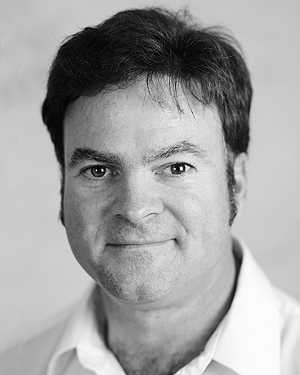
\includegraphics[width=1in,height=1.25in,clip,keepaspectratio]{a2.png}}]{Second B. Author} was
\end{IEEEbiography}

\begin{IEEEbiography}[{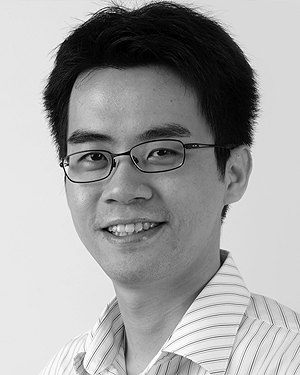
\includegraphics[width=1in,height=1.25in,clip,keepaspectratio]{a3.png}}]{Third C. Author, Jr.} l
\end{IEEEbiography}

\end{document}
